\documentclass[12pt]{article}
\setlength\headheight{14.5pt}
\title{Homework}
\author{Frederick Robinson}
\date{26 January 2010}
\usepackage{amsfonts}
\usepackage{fancyhdr}
\usepackage{graphicx}
\usepackage{amsthm}
\pagestyle{fancyplain}

\begin{document}



\lhead{Frederick Robinson}
\rhead{Math 368: Optimization}

   \maketitle

\setcounter{tocdepth}{2} 

\tableofcontents

\section{Book Problems}

\subsection{Problem 6.7a}
\subsubsection{Question}
A consumer with a utility function given by $u(x_1,x_2) = \sqrt{x_1}+x_1 x_2$  has an income of 100. The unit prices of $x_1$ and $x_2$ are 4 and 5 respectively. Compute the utility-maximizing commodity bundle, if consumption must be nonnegative.
\subsubsection{Answer}
We first note that the customer's utility maximizing bundle must cause him to expend all his money because, suppose there were some maximizing bundle which did not cause him to spend all his money, then since the utility function is strictly increasing in both $x_1$ and $x_2$ he could construct a new bundle by increasing slightly his purchase of either, constructing an affordable set with a better utility. Contradiction.

This established we reframe the problem in the following manner:
\[\mathrm{Maximize\ }\sqrt{x_1} +x_1 x_2 \ \mathrm{Subject\ to\ }4x_1+5x_2=100\]
This problem can be solved easily, either by the Lagrangian method, or by simple reduction to a one dimensional problem. I will choose the first method, so we set up our Lagrangian by 
\[L=\sqrt{x_1} +x_1 x_2+\lambda\left( 4x_1+5x_2-100 \right)\]
Now we compute each partial derivative, and set them equal to zero
\[\frac{\partial L}{\partial x_1} = 0 = \frac{1}{2 \sqrt{x_1}}+x_2+4 \lambda \quad \frac{\partial L}{\partial x_2} = 0 = x_1+5 \lambda   \]
\[\frac{\partial L}{\partial \lambda} = 0 = -100+4 x_1+5 x_2 \]
Solving this system we combine the first two equations to get 
\[  0 = \frac{1}{2 \sqrt{x_1}}+x_2-4 \frac{1}{5}x_1  \]
Then we can solve the last equation for $x_2$ and plug this in to get
\[x_2 = \frac{1}{5} \left( 100- 4 x_1 \right) \Rightarrow 0 = \frac{1}{2 \sqrt{x_1}}+ \frac{1}{5} \left( 100- 4 x_1 \right) -\frac{4}{5}x_1 \]
Simplifying this is just
\[16 x_1=5 \left(40+\frac{1}{\sqrt{x_1}}\right)\]
or, better yet
\[16 x_1=200+\frac{5}{\sqrt{x_1}}\]
solving this numerically we get
\[x_1= 12.5881 \Rightarrow x_2 = 9.92952 \]
Now, we should also check the boundary solutions, that is
\[(0,20)\quad\mathrm{and}\quad(25,0)\]
We see that
\[f(0,20)=0 \quad f(25,0)=5 \quad f(12.5881, 9.92952)=128.542\]
so indeed, our first solution is the utility maximizing bundle.


\section{Supplemental Problems}

\subsection{Problem 5.1}
\subsubsection{Question}
Find the points satisfying the first order conditions for constrained extrema and then apply the second order test to determine whether they are local maxima or local minima.
\begin{enumerate}
\item $f(x,y,z) = x y z$ and $g(x,y,z)=2 x+3 y+z =6$.
\item $f(x,y,z) = 2x + y^2 -z^2$, $g_1(x,y,z)=x-2y=0$, and $g_2(x,y,z)=x+z=0$
\end{enumerate}
\subsubsection{Answer}
\begin{enumerate}
\item The Lagrangian in this instance is given by
\[ L= x y z + \lambda \left( 2x+3y+z-6 \right)\]
We must therefore look for solutions to the following system
\[0=y z + 2 \lambda  \]
\[0=x z + 3 \lambda  \]
\[0= xy  +  \lambda  \]
\[0=2 x +3 y +z-6 \]
Solving this system reveals the following solutions
\[ \lambda= -\frac{3}{2},z= 3,x= \frac{3}{2},y= 1 \]
\[\lambda= 0,z= 0,x= 0,y= 2\]
\[\lambda= 0,z= 0,x= 3,y= 0\]
Now we check second order conditions to determine whether these are local maxima or minima.

The second order condition is checked by way of the Hessian matrix which, in this instance is given as 
\[\left[
\begin{array}{lcr}
0&z&y\\
z&0&x\\
y&x&0\\
\end{array}\right]
\] 
So for the critical points the corresponding hessians are
\[\left[
\begin{array}{lcr}
0&3&1\\
3&0&3/2\\
1&3/2&0\\
\end{array}\right]
\quad
\left[
\begin{array}{lcr}
0&0&2\\
0&0&0\\
2&0&0\\
\end{array}\right]
\quad
\left[
\begin{array}{lcr}
0&0&0\\
0&0&3\\
0&3&0\\
\end{array}\right]
\] 
Unfortunately since these matrices are indefinite the corresponding points must be saddles.
\item
The Lagrangian in this case is given by
\[ L= 2x +y^2 - z^2 + \lambda_1 \left( x-2y \right) + \lambda_2 \left( x +z \right)\]
Thus, solutions to the optimization problem must be solutions to the following system of equations
\[0=2+ \lambda_1+\lambda_2\]
\[0=2y-2 \lambda_1\]
\[0=-2z+\lambda_2\]
\[0=x-2y\]
\[0=x+z\]
We may immediately reduce the number of variables by using the last two equations to get
\[0=2+ \lambda_1+\lambda_2\]
\[0=x-2 \lambda_1\]
\[0=2x+\lambda_2\]
The first equation allows us to solve for $\lambda_1$ in terms of $\lambda_2$. Employing this relation we get a system in two variables which is easily solved.
\[\lambda_1=-2-\lambda_2 \Rightarrow 0 = x-2\left( -2-\lambda_2 \right) =x+ 4+2 \lambda_2\]
So, 
\[x=-4-2 \lambda_2 \Rightarrow -\frac{8}{3} = \lambda_2 \]
Now, substituting throughout we get
\[x= \frac{4}{3},y= \frac{2}{3},z= -\frac{4}{3}, \lambda_1 = \frac{2}{3}, \lambda_2 = -\frac{8}{3}\]

Now we need only check second order conditions to determine whether this critical point is a local minimum or maximum.

We compute the hessian matrix to be
\[\left[
\begin{array}{lcr}
0&0&0\\
0&2&0\\
0&0&-2\\
\end{array}\right]
\] 
Since this is indefinite everywhere we know that our point is a saddle.


\end{enumerate}


\subsection{Problem 6.1}
\subsubsection{Question}
Consider the problem
\[
\begin{array}{ll}
\mathrm{Maximize:} & f(x,y)=x+y\\
\mathrm{Subject\ to} & g_1(x,y) = y-2x +1 \geq 0,\\
&g_2(x,y)=x^2-y \geq 0,\\
&g_3(x,y)=1-y \geq 0 , \\
&g_4(x,y) = y \geq 0.\\
\end{array}
\]

Carry out the following steps to show that the constraint qualification fails for this problem, although a maximum exists.
\begin{enumerate}
\item \label{first} By drawing a a figure, show that the feasible set is a three sided (nonlinear) region with vertices at $(0,0)$, $(\frac{1}{2},0)$, and $(1,1)$. 
\item Add the plot of several level curves of the objective function to your figure from part \ref{first} and conclude geometrically that the point that maximizes $f$ is at $(1,1)$.
\item Show that the constraint qualification fails at $(1,1)$.

\end{enumerate}
\subsubsection{Answer}
\begin{enumerate}
\item 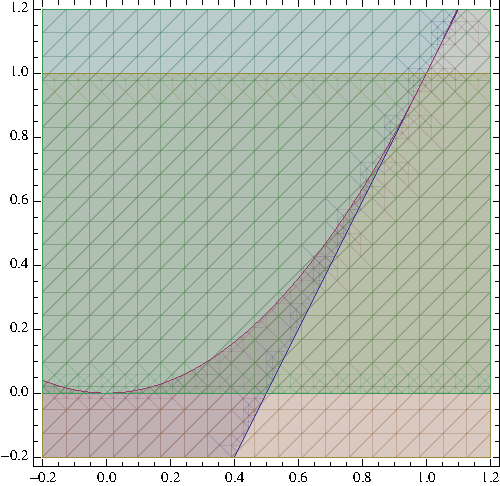
\includegraphics{region}
\item 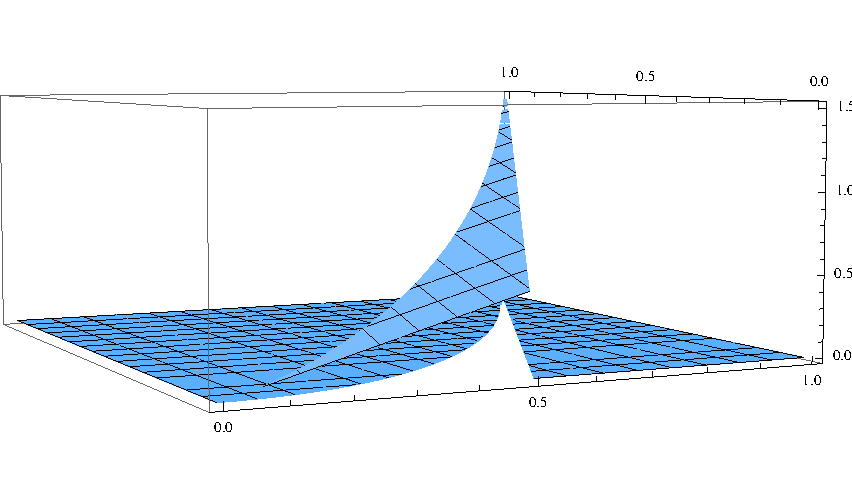
\includegraphics{height}
\item The constraint qualification fails here, because the first three constraints are effective and we get $Dh_1(x^*,y^*)=(-2,1)$; $Dh_2(x^*,y^*)=(2x,-1)=(2,-1))$; $Dh_3(x^*,y^*)=(0,-1)$. So the number of effective constraints is not equal to the linearly independent derivatives since $-(-2,1)=(2,-1)$.

\end{enumerate}

\subsection{Problem 6.2}
\subsubsection{Question}
Maximize the revenue
\[\pi = p_1 y_1 +p_2 y_2 = p_1 x_1^{\frac{1}{2}}+p_2 x_1^{\frac{1}{2}}x_2^{\frac{1}{3}}\]
subject to a wealth constraint on the inputs
\[ w_1 x_1 +w_2x_2 \leq C >0, \quad x\geq 0 \quad x_2\leq 0.\]
\begin{enumerate}
\item Write down the constraint functions and the equations that must be satisfied for the Karush-Kuhn-Tucker Theorem
\item Take $w_1=w_2=2$, $p_1=p_2=1$, and $C=8$, and find explicit values of $x_1$ and $x_2$ that attain the maximum.
\end{enumerate}

\subsubsection{Answer}
\begin{enumerate}
\item We may construct the Lagrangian as 
\[L= p_1 x_1^{1/2}+p_2 x_1^{1/2}x_2^{1/3} + \lambda \left( w_1 x_1 + w_2 x_2 - C \right) + \lambda_1x_1+\lambda_2 x_2\]
So the critical points of the problem must be solutions to
\[\frac{\partial L}{\partial x_1} = 0 = \frac{p_1}{2\sqrt{x_1}}+ \frac{p_2 x_2^{1/3}}{\sqrt{x_1}} + \lambda w_1+ \lambda_1\]
\[\frac{\partial L}{\partial x_2} = 0= \frac{1}{3}p_2x_1^{1/2}x_2^{-2/3} +\lambda w_2 + \lambda_2\]
\[\lambda \geq 0,\quad \left( w_1 x_1 + w_2 x_2 - C  \right)\geq 0,\quad \lambda \left( w_1 x_1 + w_2 x_2 - C  \right) = 0\]
\[\lambda_1 \geq 0, \quad x_1 \geq 0,  \quad \lambda_1 x_1 = 0\]
\[\lambda_2 \geq 0, \quad x_2 \geq 0,  \quad \lambda_2 x_2 = 0\]

\item We first substitute the values provided into the above equations to get
\[0 = \frac{1}{2\sqrt{x_1}}+ \frac{ x_2^{1/3}}{\sqrt{x_1}} +2 \lambda + \lambda_1\]
\[0= \frac{1}{3}x_1^{1/2}x_2^{-2/3} + 2 \lambda +\lambda_2\]
\[\lambda \geq 0,\quad \left( 2 x_1 + 2 x_2 - 8  \right)\geq 0,\quad \lambda \left( 2 x_1 + 2 x_2 - 8  \right) = 0\]
\[\lambda_1 \geq 0, \quad x_1 \geq 0,  \quad \lambda_1 x_1 = 0\]
\[\lambda_2 \geq 0, \quad x_2 \geq 0,  \quad \lambda_2 x_2 = 0\]

Since the utility function is strictly increasing in both variables we should have equality in the case of the function $ \left( 2 x_1 + 2 x_2 - 8  \right)\geq 0$ for otherwise we could increase one of the variables for a better outcome. Thus, $x_1+x_2=4$. Similarly we may set $\lambda = 0$.

So, after some algebra we attain solutions as
\[x_1= 3.2966,x_2= 0.703403,\lambda_1= 0.,\lambda_2= 0.,\lambda =  -0.382601\]

\end{enumerate}

\end{document}
